\documentclass{article}
\title{\textbf{Linux Kernel Overview}}
\author{}
\date{} 

\UseRawInputEncoding
\usepackage{graphicx}
% Links
\usepackage{hyperref}
\hypersetup{
    colorlinks=true,
    linkcolor=blue,
    filecolor=magenta,      
    urlcolor=cyan,
}
 
\urlstyle{same}

% Code Coloring
\usepackage{xcolor}
\usepackage{listings}
\lstset{
  language=bash,
  basicstyle=\small\sffamily,
  showstringspaces=false
  %numbers=left,
  %numberstyle=\tiny,
  numbersep=3pt,
  %linewidth=13cm,
  frame=tb,
  columns=fullflexible,
  backgroundcolor=\color{yellow!20},
  linewidth=0.9\linewidth,
  xleftmargin=0.1\linewidth
}


%Box Note
\usepackage{graphicx}
\usepackage{tcolorbox}
\tcbuselibrary{skins}
\usepackage{lipsum}
\definecolor{boxTitle}{HTML}{fff79a}
\definecolor{boxBackground}{HTML}{fffce0}
\definecolor{boxFrame}{HTML}{f1e2b8}

\tcbset{my box/.style={
    enhanced, fonttitle=\bfseries,
    colback=boxBackground, colframe=boxFrame,
    coltitle=black, colbacktitle=boxTitle,
    attach boxed title to top left={xshift=0.3cm,
                                    yshift*=-\tcboxedtitleheight/2},
    boxed title style={
      before upper=\hspace*{0.5cm}, % reserve space for the image
      overlay={
       \node at ([xshift=0.5cm]frame.west)
         {\includegraphics[scale=0.65]{bc-dodecaedre}};
      }
    }
  }
}

\newtcolorbox{mybox}[1][]{my box, #1}

\begin{document}
\maketitle
\tableofcontents{}
\section{What is the Linux kernel ?}

Q: Where to find the Linux Kernel ?\\
A: You can find it under \textbackslash boot, you will find "vmlinuz-xxx" (FYI: vmlinuz the z means compressed image, vmlinux is not compressed !)

\subsection {Linux Important concepts}
\begin{itemize}
    \item each application has a specific use, and programs should not do more than what it's supposed to do. (one program = one function only), and you can reach the overall functionality by letting the applications cooperate together.
    \item Everything is a file !
    You need to know that Linux deals with everything as a file to read/write from and into it. and you have seven types of a files as following:
    \begin{enumerate}
        \item - : regular file
        \item d : directory
        \item c : character device file
        \item b : block device file
        \item s : local socket file
        \item p : named pipe
        \item l : symbolic link
    \end{enumerate}
    And you can get the type of a certain file by using the \textit{ls -ld <file name>}
    \lstinputlisting[caption=HW info]{./resources/src/everythingisafile}

\end{itemize}

\section{Understanding the \textit{syscalls}}
They are some functions implemented by the kernel for the user space to request operations from the kernel. there are around 400 Linux \textit{syscalls}.\\
You can find the list of them in \textbf{``include/uapi/asm-generic/unistd.h"} in the Linux kernel source tree. in this file, you will find some constants which every constant is a system call id.

When you use a system call to ask the kernel to do something for you, the parameters will stored in a registers and the kernel is invoked (through a software interrupt), then it determines which call call is invoked, and call it.
according to the system call return value you can continue your application, but if the system call returned -1, and you should handle that error as per your application. let's see an example:

\lstinputlisting[caption=HW info]{./resources/src/syscall-read-man}

as you can see for the read \textit{syscall}, it returns the number of bytes read or otherwise if there is an error, it returns -1.\\

\subsection{Defining your own \textit{syscall}}
\begin{enumerate}
    \item Add a constant for the syscall APIs in \textbf{"/arch/x86/include/asm/unistd\_32.h"} to have a new entry for the syscall
        \lstinputlisting[caption=Add the syscall constant "/arch/x86/include/asm/unistd\_32.h"]{resources/src/syscall/1.syscall_cont}
    
    \item Define the syscall definition in "linux/arch/x86/include/asm/syscalls.h" (note: define it according to the target architecture x86\_x64 or x86) 
    Define the function with the standard naming conversion sys\_ to identify it as sys call
    \lstinputlisting[caption=Define the syscall definiation "linux/arch/x86/include/asm/syscalls.h"]{resources/src/syscall/2.signature}

    \item Define the switch table for the call
    \item Define the syscall in the syscall switch table "/arch/x86/kernel/syscall\_table\_32.S"
    The switch table which the addresses are called
    
    \begin{center}
        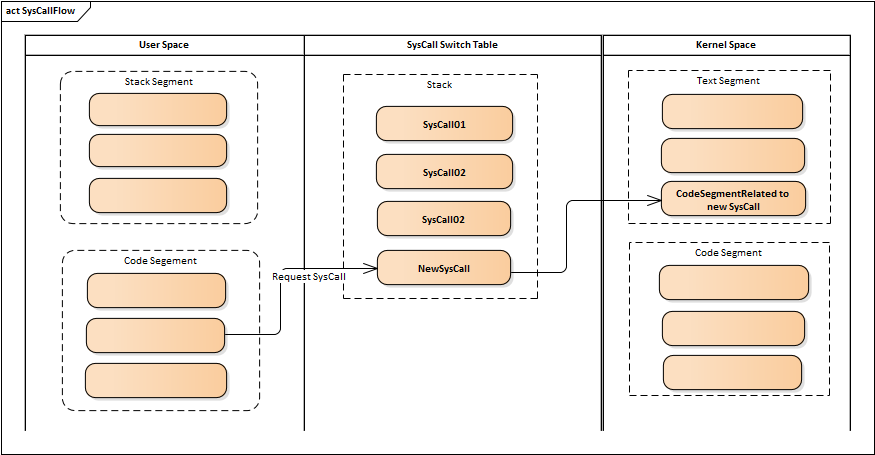
\includegraphics[scale=0.60]{./resources/img/new_syscall.PNG}
    \end{center}

    \item Add the implementation in any file (no rules), you can create your own .C file for your own call
    Let's implement it in \textbf{"/kernel/sys.c"}
    \lstinputlisting[caption=syscall implementation "/kernel/sys.c"]{resources/src/syscall/4.syscall_implementation}

    \item Build the kernel
\end{enumerate}

\subsection{Steps to call a system call from the user space}
\begin{enumerate}
    \item Copy system caller ID to eax (int) accumulator
    \item Starting with right most argument and move each parameter onto each accumulator starting with ebx (max of 6 accumulator in intel)
    \item Initiate a trap exception using processor specific instruction
    \item read the exit value of the system call for eax.
\end{enumerate}

The system call handling (as well the exception handling) is handled in \textbf{"/arch/i386/kernel/entry.S"}
this file would be handled as follow
\begin{itemize}
    \item Reads EAX
    \item lookup syscall switch table (the offset of the function)
    \item Allocate kernel stack (store the local data in the kernel stack)
    \item Update EIP register in PCB
\end{itemize}

These steps are converting the code from the user mode to kernel mode with more privileges
\lstinputlisting[caption=Syscall handling]{resources/src/syscall/6.handling-syscall}


\begin{mybox}[title={Difference between a normal function call and a syscall}]
     \begin{itemize}
         \item Function call
         \lstinputlisting[caption=Normal function call]{resources/src/syscall/4A.functioncall}

         \item Invoking a system call
         \lstinputlisting[caption=Invoking syscall]{resources/src/syscall/4B.syscall}

     \end{itemize}
\end{mybox}

You might read about the exception handling topic, \href{https://www.kernel.org/doc/html/latest/x86/exception-tables.html}{here}.

\subsection{The system calls and the c Library}
To make the application level code architecture independent, the use of the C Library is raised, as the C Library will be the translation unit(interface) between the kernel and the application, and for sure the C Library itself uses the system calls, and as an application developer you can use the C Library or directly use the Kernel \textit{syscalls} to create applications.

\begin{center}
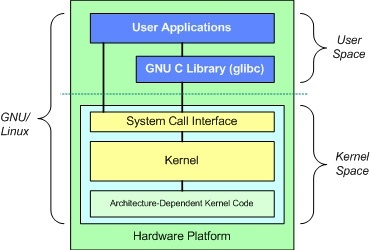
\includegraphics[scale=0.75]{resources/img/libclang-linux}
\end{center}
And you should know that the \textit{syscalls} are unique by the system.

\subsection{Controlling and viewing information about the HW}
As demonstrated above, You can use some applications to collect or even to control the HW devices.\\
These applications uses some C library functions, which used the kernel \textit{syscalls} to control or display these information.
Lets's see an example; \textit{lshw, lspci, lsusb, lsblk, lscpu, lsdev}\\
for example if we used the \textit{lspci} we will find that the terminal displays info about all the connect PCI devices 

\lstinputlisting[caption=HW info]{resources/src/hw-info}

\textbf{Note:} that you can use lspci -v for the verbose mode (i.e. more information)\\

Even you can control the HW using the following command: \textit{hdparm} or \textit{setpci} commands
\lstinputlisting[caption=HW Control]{resources/src/hw-control}
You can use also other approach to control the HW units using the Linux \textit{virtual file system}
like echo to proc, dev, or sys file systems.

\subsection{Reading the kernel messages!}
\textit{printk} is the kernel function to print messages, it's like C's printf() but for the kernel. the messages by \textit{printk} is sent to a RAM buffer and sometimes to the system console.
the kernel used a Logging Daemon to send the messages to a file or somewhere else. if you want to display these messages you can use the command \textit{demesg}. it displays theRAM buffer to your terminal, and you need to note that the messages starts from very early of the boot process.
\lstinputlisting[caption=The Linux File System]{resources/src/log-dmesg}

You can also display some messages by accessing this file /var/log/messages or /var/log/syslog
use: \textit{tail -f /var/log/messages}

\subsection{The virtual file systems}
/proc and /sys files systems don't store their file system on the disk permanently, they generate it every time the Kernel runs or when you ask for it.
it's not like the RAM file system, as the RAM file system stores their contents in the RAM.

\begin{enumerate}
    \item /Proc - coming from process, and it's mounted at the boot time.
        it contains all the information of the running processes, and you can use the \textit{\textbf{ps}} (process status) command to get the information you want from the \textit{proc} file system.
        every process has a unique id PID, and there are files and directories per process.
        the process threads is represented in a process subdirectory called 'task'

        \lstinputlisting[caption=The proc file system]{resources/src/theprocfs}
        As you might noticed, They are normal text files.\\
        
        as you can consider the system as a process under \textit{/proc}, then you can modify the system behavior in boot time or at runtime using the system tunable parameters (to tune the kernel). the \textit{/proc/sys} file system contains all of them.
        For example searching for ip\_forward tunable variable. you will find this variable underneath "./sys/net/ipv4/ip\_forward", and it's value is 0 which means ip forwarding is not working.
        \lstinputlisting[caption=Tunable variables]{resources/src/tunable-vars}

        Note: use the cat command to print a file, while echo to set into it.

        You can use the command sysctrl to print all the tunable variables.
        \begin{lstlisting}
            ubuntu@ip-172-31-46-156:~$ sysctl -a
            abi.vsyscall32 = 1
            debug.exception-trace = 1
            debug.kprobes-optimization = 1
            dev.cdrom.autoclose = 1
            dev.cdrom.autoeject = 0
            ...

            ubuntu@ip-172-31-46-156:~$ sysctl -a | grep ip_forward 2>/dev/null
            net.ipv4.ip_forward = 0
            net.ipv4.ip_forward_use_pmtu = 0

        \end{lstlisting}

        You have to notice that you should use the \textit{sysctl} command to deal with the tunable parameters. for example:

        or you can change the Linux tunable parameters permanently by writing to the \textit{/etc/sysctl.conf} file.
        \lstinputlisting[caption=The proc file system]{resources/src/sysctl-write-panic}

        Note: The Linux tunable parameters can be used for Linux kernel optimization or to change the Linux behavior at runtime or during initialization.

    \item /sys 
        it's mounted at boot time, and it is for the 'kernel object' info.
        it contains info about the the connected HW (e.g. PCI info)

        \lstinputlisting[caption=The \textit{sysfs}]{resources/src/thesysfs}

\end{enumerate}

\section{The device files}
Device files, are used for two kinds of devices; character or block devices.
each device file have a major number, minor number, and a character to represent if it's block (b) or character (c).
and you can interact with the a device by using its device files.
the major numbers is used for all the same kind of devices, but the minor number is unique per a device.
for example if you have a serial devices, then expect that they will all have the same major number.

The mounting point if the devfs is the /dev node.

\subsection{Dealing with a device file}
for example the character device files can implement read(), write(), and ioctl(), while enables then to deal with the device files.
so a process opens a device file which returns a file descriptor then to use these implemented functions to access the device files.

\lstinputlisting[caption=Access a device file]{resources/src/devicenull}
The kernel will arrange to call the write() function for the \textit{null} device file 

Note: in Linux, the \textit{/dev/null} is called the null device file which is absorbing any data written or redirected to it (the Linux black hole), you can use it to ignore info while displaying a certain needed info only.
Also there is /dev/zero while a character device file considered an source of zeros, and /dev/random and /dev/urandom which an infinite source of random number (used as a secure source of random number for crypto-systems)

\lstinputlisting[caption=Access a device file]{resources/src/devicenull-usageex}

The following example throw all the stderr output to the null!, try it without using the \textit{/dev/null}.

In the following example, you can check your internet speed without occupying your disk!. 
\lstinputlisting[caption=Access a device file]{resources/src/devicenull-usageex2}

\subsection{The block devices}
To see the block devices you have, change your directory to \textit{/sys/block}.
\lstinputlisting[caption=Access a device file]{resources/src/block-devices}

You can use the fdisk command to check all the attached HDDs. use \textit{sudo fdisk -a}

\subsection{The Linux file system}
Linux file system is single tree (unified file systems hierarchy), And you can install this tree distributed on multiple storage devices\\
So you have primary partition (contains root), and you can have one or more mounting points on disk.
The file system hierarchy is as follow:
\begin{itemize}
    \item / - the root node (it called slash/)
    \begin{itemize}
        \item /root - home directory for root user fs(admin). You need permissions to access.
        \item /boot - Contains all boot files needs boot the system 
        \item /home - contains all the users of the system, you can also reach your home using the ~ sign from the command line
         grub - contains the bootloader, its binary, configs for boot, and kernel image e.g. vmlinuz-4.15.0-1051
        \item /bin - contains all the command line applications
        \item /lib - contains the shared libs
        \item /etc - contains all configuration files for all the programs
        \item /dev   - its a placeholder for all devices in the system (Linux deal with any devices as files to read and write as buffer)
        \item /media - the mounted devices (camera, sdcard, ...)
        \item /mnt  - the mounted devices (camera, sdcard, ...)
        \item /opt  - Optional software
        \item /usr  - Shared data or binaries among all users
        \item /var  - variable files or log files ...
        \item proc  - the proc file system is used to hold all the running processes 
        \item sys   - Interface for kernel 
    \end{itemize}      
\end{itemize}

\lstinputlisting[caption=The Linux File System]{resources/src/thefs}

\section{Linux Boot Process}
GRUB is the Linux boot loader, the BIOS loads GRUB and GRUB loads the kernel image into memory.\\

GRUB loads the kernel and the \textit{initfs}, and setup the kernel command line, then transfer the control to the kernel after passing the command line parameters to it.
GRUB is built with support of file systems, it can find files, and can load the kernel by name, it can also find the kernel by its file name completion feature.\\

Note: use \textit{man -k grub} to see more about GRUB features.


\subsubsection{The passed command line parameters}
GRUB passes the command line parameters to the kernel. so that you can put a script to handle during booting.
You can access these command lines by using \textit{dmesg} or by using \textit{/proc/cmdline}.

For a documentation about the kernel parameters, you will find in the Linux source tree in \textit{documentation/kernel-parameters.txt}

\subsubsection{The init file system}
The initial file system or it's called the RAM file system (initrd) is used to provide drivers and support for mounting the system's real file system. 
The \textit(initrd) has the init task which responsible for loading the device files which enables the Kernel to load the real file system.
after init in \textit{initrd} terminates, the kernel will start again the real init again this time from the real file system on disk.
this init in Linux is called a \textit{\textbf{systemd}}. this init fs starts the Linux daemons after initializing the kernel. and the configuration of these services is under \textit{/etc/systemd/system}.

\lstinputlisting[caption=The Linux File System]{resources/src/booting/init-prog}


You can find the initramfs in \textit{/boot/init/initrd}, it's a CPIO zipped file, the Linux will extract it and mount it into RAM.
to explore its internals and know about the services inside it. you can do the follow:

\lstinputlisting[caption=The Linux File System]{resources/src/booting/extract-initrd}


Note: Booting the system with rdinit=/bin/sh it will start a shell within initramfs. but If you start using init=/bin/bash it will start a bash after the initramfs is completed from the real file system on the disk.
refer to \hyperref[sec:interrupt-grub]{Interrupting GRUB}

\subsection{Configuring GRUB}
You can configure GRUB V1 by editing the \textit{grub.conf} to add kernel entries
In GRUB V2 there is a complete directory for that \textit{/etc/grub.d}, also you can find \textit{/etc/default/grub} for the default configuration.
In order to have a new grub entry, you can add a file under \textit{/etc/grub.d}.\\

after adding any entries, then you need to call \textit{update-grub} to update grub with the new info.

You can edit the \textbf{40\_custom} file in \textit{/etc/grub.d} to easily add a new kernel entry.

\lstinputlisting[caption=The Linux File System]{resources/src/booting/add-grub-entry}

you can notice that we put \textbf{initcall\_debug} as a part of our menuentry, so after rebooting, you can type \textit{dmesg | initcall} and it will show all the log of init and order of executing and loading of the devices. then you can analyze and debug the init task. 

\subsection{Interrupting GRUB}
\label{sec:interrupt-grub}
Normally you can do that by pressing any key while booting. and then temporarily edit the GRUB configurations.

You can then press 'P' (GRUB 1) or Ctrl+'x' (GRUB 2) to resume booting.

You can also overriding the initrd; 
\begin{enumerate}
    \item reboot the system
    \item after rebooting hit the down arrow to interrupt GRUB
    \item then select any kernel entry, then type 'e' to edit its configurations.
    \item the configuration will appear, just add at last \textit{init=/bin/bash}. what do you notice?
    You will see that we have overridden the \textit{initrd} and just jumped to the real fs on disk.
\end{enumerate}
<<Photo here from reboot>>

\section{Building the Linux kernel}
You need first to get a kernel version from \href{https://kernel.org/pub/linux/kernel/}{the kernel official website}.

\begin{enumerate}
    \item Get the Linux kernel source code:
        wget https://mirrors.edge.kernel.org/pub/linux/kernel/v5.x/linux-5.3.15.tar.xz
    \item Un-tar it: 
        tar xf archive.tar.xz
    \item You can use \textit{\textbf{make menuconfig}} or \textit{\textbf{make xconfig}} to configure the kernel.
    All the configurations will be stored in the \textit{.config} file
    \item Then you can use different targets to build the kernel; \textit{make bzimage}, \textit{make modules}, \textit{make install}, \textit{make modules\_install}, or \textit{make clear}.
\end{enumerate}

Note: You can use \textit{make help} to guide your about the targets of the makefile.

\subsection{kernel patches}

\section{The loadable kernel modules (LKM)}
They are .ko (kernel objects) files which \textbf{dynamically} adds more functionality to the kernel itself, and they run in the kernel space. 
So you can add a functionality to the kernel when you need without editing the kernel. and keeps the kernel with small size.

So where to find the kernel modules, simply in \textit{/lib/modules}

\lstinputlisting[caption=The Loadable Kernel Modules]{resources/src/lkms/cd-modules}

and you will find also some configuration files at the same directory.

the modules can be at any directory, but the \textit{modprobe} is designed to look only in \textit{/lib/modules}.

Note the LKM should complied to a certain kernel version not the other.

\subsection{LKMs Commands}
\begin{itemize}
    \item The \textit{lsmod} will list all the loaded module with its usage and its dependencies, if a modules depend on another modules, then the last one must be loaded before the new one otherwise an error will appear.
    \lstinputlisting[caption=Lisiting the kernel modules]{resources/src/lkms/lsmod}
    \item The \textit{rmmod} will remove a module, and take care when removing a module which already in use, It can panic the kernel.\\
    \item The \textit{modinfo} will print t a meta-data about the module; name, author, or parameters, aliases, ... .
    \item The \textit{depmod} will create file for the dependencies of the modules ("modules.dep" file in \textit{/lib/nodules/KER\_VER}).
    \item The \textit{insmod}, and it returns after the module initialization done. (don't use and use \textit{modprobe} instead)
    \item The \textit{modprobe} load a module and looks for its dependencies which are generated from \textit{depmod}
    Note: \textit{modprobe} can do other operations on the modules.

\end{itemize}

\subsection{Creating and Building a simple kernel module}

A simple loadable kernel module:
\lstinputlisting[caption=A source of a simple LKM]{resources/src/lkms/simple_module/simple_module.c}

\lstinputlisting[caption=A source of a simple LKM]{resources/src/lkms/simple_module/building_bash}


\subsection{Developing Device Drivers by LKMs}

\section{Little bit about the application development}

In Linux, as an application developer you can develop your application in "C" in different ways:
\begin{itemize}
    \item Using the Linux \textit{syscalls}
    \item Interfacing the \textit{syscalls} by the libc.
    \item Or you can use an application framework like QT to even develop a beautiful GUI applications 
\end{itemize}

\subsection{Meet Vim, GCC, and GDB}
Vim is the command line text editor in Linux, it's very powerful tool to edit the text files without any GUI interface.\\
Why to use Vim ?\\
In embedded systems developments and debugging, you might not having the facility to edit the files using a full featured text editor over terminal.\\ 

Vim Modes:
\begin{itemize}
    \item Text Mode
    \item Command Mode
\end{itemize}

Note: for multiple files projects you might need to use \textit{make} or \textit{cmake} to manage your building process.


\subsubsection{GDB - The GNU Debugger}
First you need to compile your code using debug symbols as follow, and note that you can use \textit{-g or -ggdb} for a gdb format, also you can choice the level of the debugging info by specifying -g1, -g2, or -g3:\\
\textit{g++ -g example.cpp -o output.exe}

Sometimes, people choice -O3 while compiling for optimization level3, if you use \textit{-O3 -g} but the information while debugging will be poor.\\

In order to use GDB, you can run the following command, \textit{gdb -q ./output.exe}, as you can see in the following example, you can find that gdb is working
\lstinputlisting[caption=Running the GDB]{resources/src/gdb/1-start-debug}

You can make several operations using gdb, you need to set a break point, and then type run, gdb will stop at the break point:
\lstinputlisting[caption=GDB Basic Operations]{resources/src/gdb/2-set-break}

Now you can type some commands to GDB to explore the memory, and here is some examples:
\begin{enumerate}
    \item \textit{info registers} can be used to list all the register, you can also to get a value inside a certain register
    \lstinputlisting[caption=Working with registers]{resources/src/gdb/3-info-reg}
    
    \item \textit{"x" short for examine} is used to have direct access to the memory, it's used to display the memory. you can examine in different formats
        \begin{itemize}
            \item o Display in octal.
            \item x Display in hexadecimal.
            \item u Display in unsigned, standard base-10 decimal.
            \item t Display in binary.
        \end{itemize}

    The \textit{"x"} is very powerful as it can explore the memory in a lot of ways, let's have some examples:

    \lstinputlisting[caption=Display a memory locations]{resources/src/gdb/examine-memory}

    as you can see, we displayed the memory of the next instruction stored in \textit{rip} register, even you can reference the register to it the address stored on it using \textit{\$rip}, and for all times the outputs is the same but in different formats.\\
    
    Even you can display the memory in different sizes, as the default examine size if \textit{word}, then you have other ways to how the memory is treated and this can be useful in certain locations:

    \lstinputlisting[caption=Change the size of printed data]{resources/src/gdb/examine-memory02}

    \begin{itemize}
        \item A single byte
        \item h A halfword, which is two bytes in size
        \item w A word, which is four bytes in size
        \item g A giant, which is eight bytes in size
    \end{itemize}

    As the gdb is used also to disassemble the code, then you can use the "x" command to display the disassembled instructions, hence you can use "x" instruction to display the number of disassembled instructions as follow:
    \lstinputlisting[caption=Display a memory locations]{resources/src/gdb/examine-memory03}
    
    One hint: in GDB you can use a full text commands or you might need to write a abstracted commands, see the example below, instead of writing \textit{"info register rip"}, \textit{"i r rip"}, and they will give the same result. 
    \lstinputlisting[caption=Write your GDB instructions in an easy way]{resources/src/gdb/cmd-summary}


\end{enumerate}

\subsubsection{Creating GDB Scripts}
A good thing when you use GDB is that you can setup a script to run as a debugging scenario, and let it get the debugging info you needed for you.\\

By default during startup, gdb executes the file \textit{.gdbinit}. This is where you write your gdb code. In case you want to have many scripts that test different things, you can tell gdb to look at other scripts besides the default one by adding the \textit{--command=<filename>} argument when running gdb.\\

by writing \textit{\textbf{gdb -q --command=backtrace-script}}, you will get trace of all frames in stack of our program:
\lstinputlisting[caption=backtrace script output]{resources/src/gdb/gdb-backtrace-output}

and the script is:
\lstinputlisting[caption=backtrace script]{resources/src/gdb/gdb-backtrace-script}

for more info, you can refer to the gdb quick reference from \href{http://users.ece.utexas.edu/~adnan/gdb-refcard.pdf}{here}.
\subsection {Concurrent Programming}
You can achieve concurrent programming in Linux using two ways:
\begin{itemize}
    \item Kernel Level threads
    Kernel-level threads are handled by the operating system directly and the thread management is done by the kernel. The context information for the process as well as the process threads is all managed by the kernel.

    \item User Threads using threads library (pThreads), or C++ threads using C++ thread library
    The user-level threads are implemented by users and the kernel is not aware of the existence of these threads. It handles them as if they were single-threaded processes. User-level threads are small and much faster than kernel level threads.
\end{itemize}


\subsubsection {Linux Threads}
You can create a kernel level threads in two ways; Using fork(), or clone() system calls, but before let's have a look on how threads works in the different OSs:\\
In windows:\\
- it will create a PCB, Process Control Block (in the kernel space) related to that PID and points to the main process of that program, when the processor starts a new thread 
- it's allocates a new dynamic memory and puts this code into it and creates a new thread object which points into it (with the same PID)
- The key point now is whatever the CPU time acquired by this PCB (represent the main program), that has to be shared on these threads, and the piece of code which will divide this time among the threads called -> user level scheduler
and if we need more time to be allocated for a certain thread, we need to change it's priority, note that the kernel scheduler is not aware of the contexts or threads in the user space, the object that holds an info about the thread is called thread object
- For each thread -> ThreadObject, + Code + Stack
- but the issue of that model is, that the user space scheduler is not performing a full context switching but when the time of a thread ends, the user space scheduler just will move the control o the other thread, it's conditional jump to the other thread

In Unix based thread:\\
- A new address space in the user space will be allocated for every thread,
- A new PCB address space in the kernel space will be allocated to point on every thread, every thread is a new process (with differnet PID) identified by the kernel 
- The difference now is all the info about the threads will be allocated in the PCB related to that thread in the KERNEL SPACE with the control of the kernel
- This kind of threading is called kernel supported threading

-In the matter of performance windows is good (because switching between thread is just a conditional jump and no context switching), in the matter of fault tolerance, linux is better
-Comparing the programmers friendly for each one, the easy to debug and the easy to deal with is the user threading module in windows is more friendly because a global varaibles is not accessible anymore in linux after creating a threads to share data, the same is not here in unix
to exchange data between thread, the developer should write extra code for sharing between them this called interprocess communication IPC!
- In the matter of distrusting the thread between cores, Unix based are better because in user level threading, you have all the threads within the same PCB then they share the same core,
but for the Unix based it's possible to have thread1 in a core, thread2 in another core ...

But Linux came with the best of two approaches, LWP Light-Weight Process, Linux got a concept of clone in place of fork,
clone will create a new address space  as fork exactly, but it will allow a the processes o share resources with parents and now they can access the globle data in data segement or file descriptors for the parent, which means no need for IPC anymore.\\

Using fork():\\
fork -> sys\_fork -> do\_fork
- all the resources in the parent PCB are copied into the child PCB
- After the child process terminates, the parent process should read its exit, if not the child enters a state called zoombie state or defunct state
- every process enters this state !, at this moment the PCB for this process is still exists, and all the resources for it are locked up, when all processes are in zoombie, the system is frozen coz all resources locked up
- There are two approaches to notify the parent about exit
1. Sync  - suspend the parent till the child terminates
2. Async - Child sends a signal to the parent\\

What is happening with fork() ?\\
- parent's page tables(PCB, and address space, stack, global, and local data) been copied to child to create a unique task structure for the child!
- But this is not right, actually what happens, that the Linux makes a Copy-On-write ONLY, means that the resources shared with parent are read-only, and when acquire to write, the linux will copy this portion in memory and write into it

\lstinputlisting[caption=Consumer Producer example]{resources/src/threads/fork-example}

Clone system call:\\
It is used to create multiple threads that can concurrently run in the same shared memory space!, clone is the same fork(), but you control the resources you share with child

You can create threads using clone as following:
pid\_for\_child = clone(funn\_pointer\_for\_the\_child, stack+stack\_size, flags, any\_args\_passed\_to\_child)

\subsubsection{POSIX Threads (pthreads)}
On the other side, you can use the POSIX thread to create a user-level threads. and this example as a simple thread:
\lstinputlisting[caption=Simple pThreads example]{resources/src/threads/pthreads/pThreadsExamples/pthreads-simple}

The difference between threads and fork, fork creates another process which has its own PDT (Process Descriptor table) but Pthreads sharing the same PDT
Note: pthreads APIs use clone syscall

You can use also use a synchronization methods like mutex and conditional variables as follow:
\lstinputlisting[caption=Consumer Producer example]{resources/src/threads/pthreads/pThreadsExamples/Semaphores/Semaphores_ProducerConsumerProblem_Semaphore.c}


\subsubsection{C++ Threads (C++11 and C++14)} 
Here is a simple example of creating a simple thread
\lstinputlisting[caption=A source of a simple LKM]{resources/src/threads/cpp_threads_example01}

\subsubsection{Socket Programming}

\subsubsection{Linux Application Development}

\subsubsection{Meet Gnome GDK+ and KDE QT}

\section{Installing Ubuntu distribution}
While installing, how to partition your hard disk

\section{Bash Scripting}


\section{some useful commands}
1. Check the kernel version; use the uname command (unix name)
\begin{lstlisting}
    ubuntu@ip-172-31-46-156:~$ uname -r
    4.15.0-1057-aws
    ubuntu@ip-172-31-46-156:~$    
\end{lstlisting}

2. check the memory usage, you can use the procfs
\begin{lstlisting}
ubuntu@ip-172-31-46-156:~$ head /proc/meminfo
MemTotal:        1007300 kB
MemFree:          351080 kB
MemAvailable:     734812 kB
Buffers:           32956 kB
Cached:           438592 kB
SwapCached:            0 kB
Active:           361348 kB
Inactive:         160464 kB
Active(anon):      50860 kB
Inactive(anon):      164 kB
ubuntu@ip-172-31-46-156:~$
\end{lstlisting}

3. use the strace command (\textit{syscall} trace) to check the usage of an application to the system calls
Example: make a report of usage of the syscalls for date command 
\lstinputlisting[caption=The Linux File System]{resources/src/strace-cmd}

the date command prints the date and uses for that a system calls, we use strace with the option -c (count) to count the usage of the \textit{syscalls}.

4. Search for all the device files with the same major number.
for example, /dev/null has the major number 1, and minor number 3 as follow, then we can use grep to get all the device files ``\textasciicircum c" then to match again all the device files with major number 1.
\lstinputlisting[caption=Lisiting all the device files with the same major number]{resources/src/useful-commands/getalldeviceswithmajornumber}

5. The pstree command\\
it prints a tree for all the relationship of the processes.
\lstinputlisting[caption=The first process in pstree command]{resources/src/utils/pstree}

6. The systemctl - working with the \textit{systemd} services
The command used to check if a systemd daemon (or service) is running

\lstinputlisting[caption=Lisiting all the device files with the same major number]{resources/src/systemd/check-service}


You can use also use the \textit{ps} command indirectly to see if the sshd service is running as one of the process as shown.

\subsection{But what is systemd ?}

7. Using cat command to append into files, just use <<EOF>> with cat. then write what ever you want and when you type EOF it will exit!.
\lstinputlisting[caption=Cat to append on text files]{resources/src/linux-commands/working-with-files/cat-append}

8. History command for shell, it get's use all the commands you run on your bash and you can configure it to keep as much history as you can
\lstinputlisting[caption=History Command]{resources/src/linux-commands/misc/history-command}

9. working with files and directory using \textit{chmod}
\lstinputlisting[caption=File Permissions using chmod]{resources/src/linux-commands/working-with-files/chmod}

You can use also \textit{umask} command which allows you to view or to set the file mode creation mask, which determines the permissions bits for newly created files or directories.
It is used by mkdir, touch, tee and other commands that create new files and directories.
\lstinputlisting[caption=File Permissions using umask]{resources/src/linux-commands/working-with-files/umask}

and you can change the ownership using \textit{chown}:
\lstinputlisting[caption=ownership Control]{resources/src/linux-commands/working-with-files/chown}

Understanding the ACL (Access Control Lists)
\lstinputlisting[caption=getfacl and setfacl]{resources/src/linux-commands/working-with-files/acl}


\end{document}